\newcommand{\figwidth}{1.0\textwidth}

\begin{figure*}[ht!]
\vspace{-15pt}
\centering
\captionsetup{width=\figwidth}
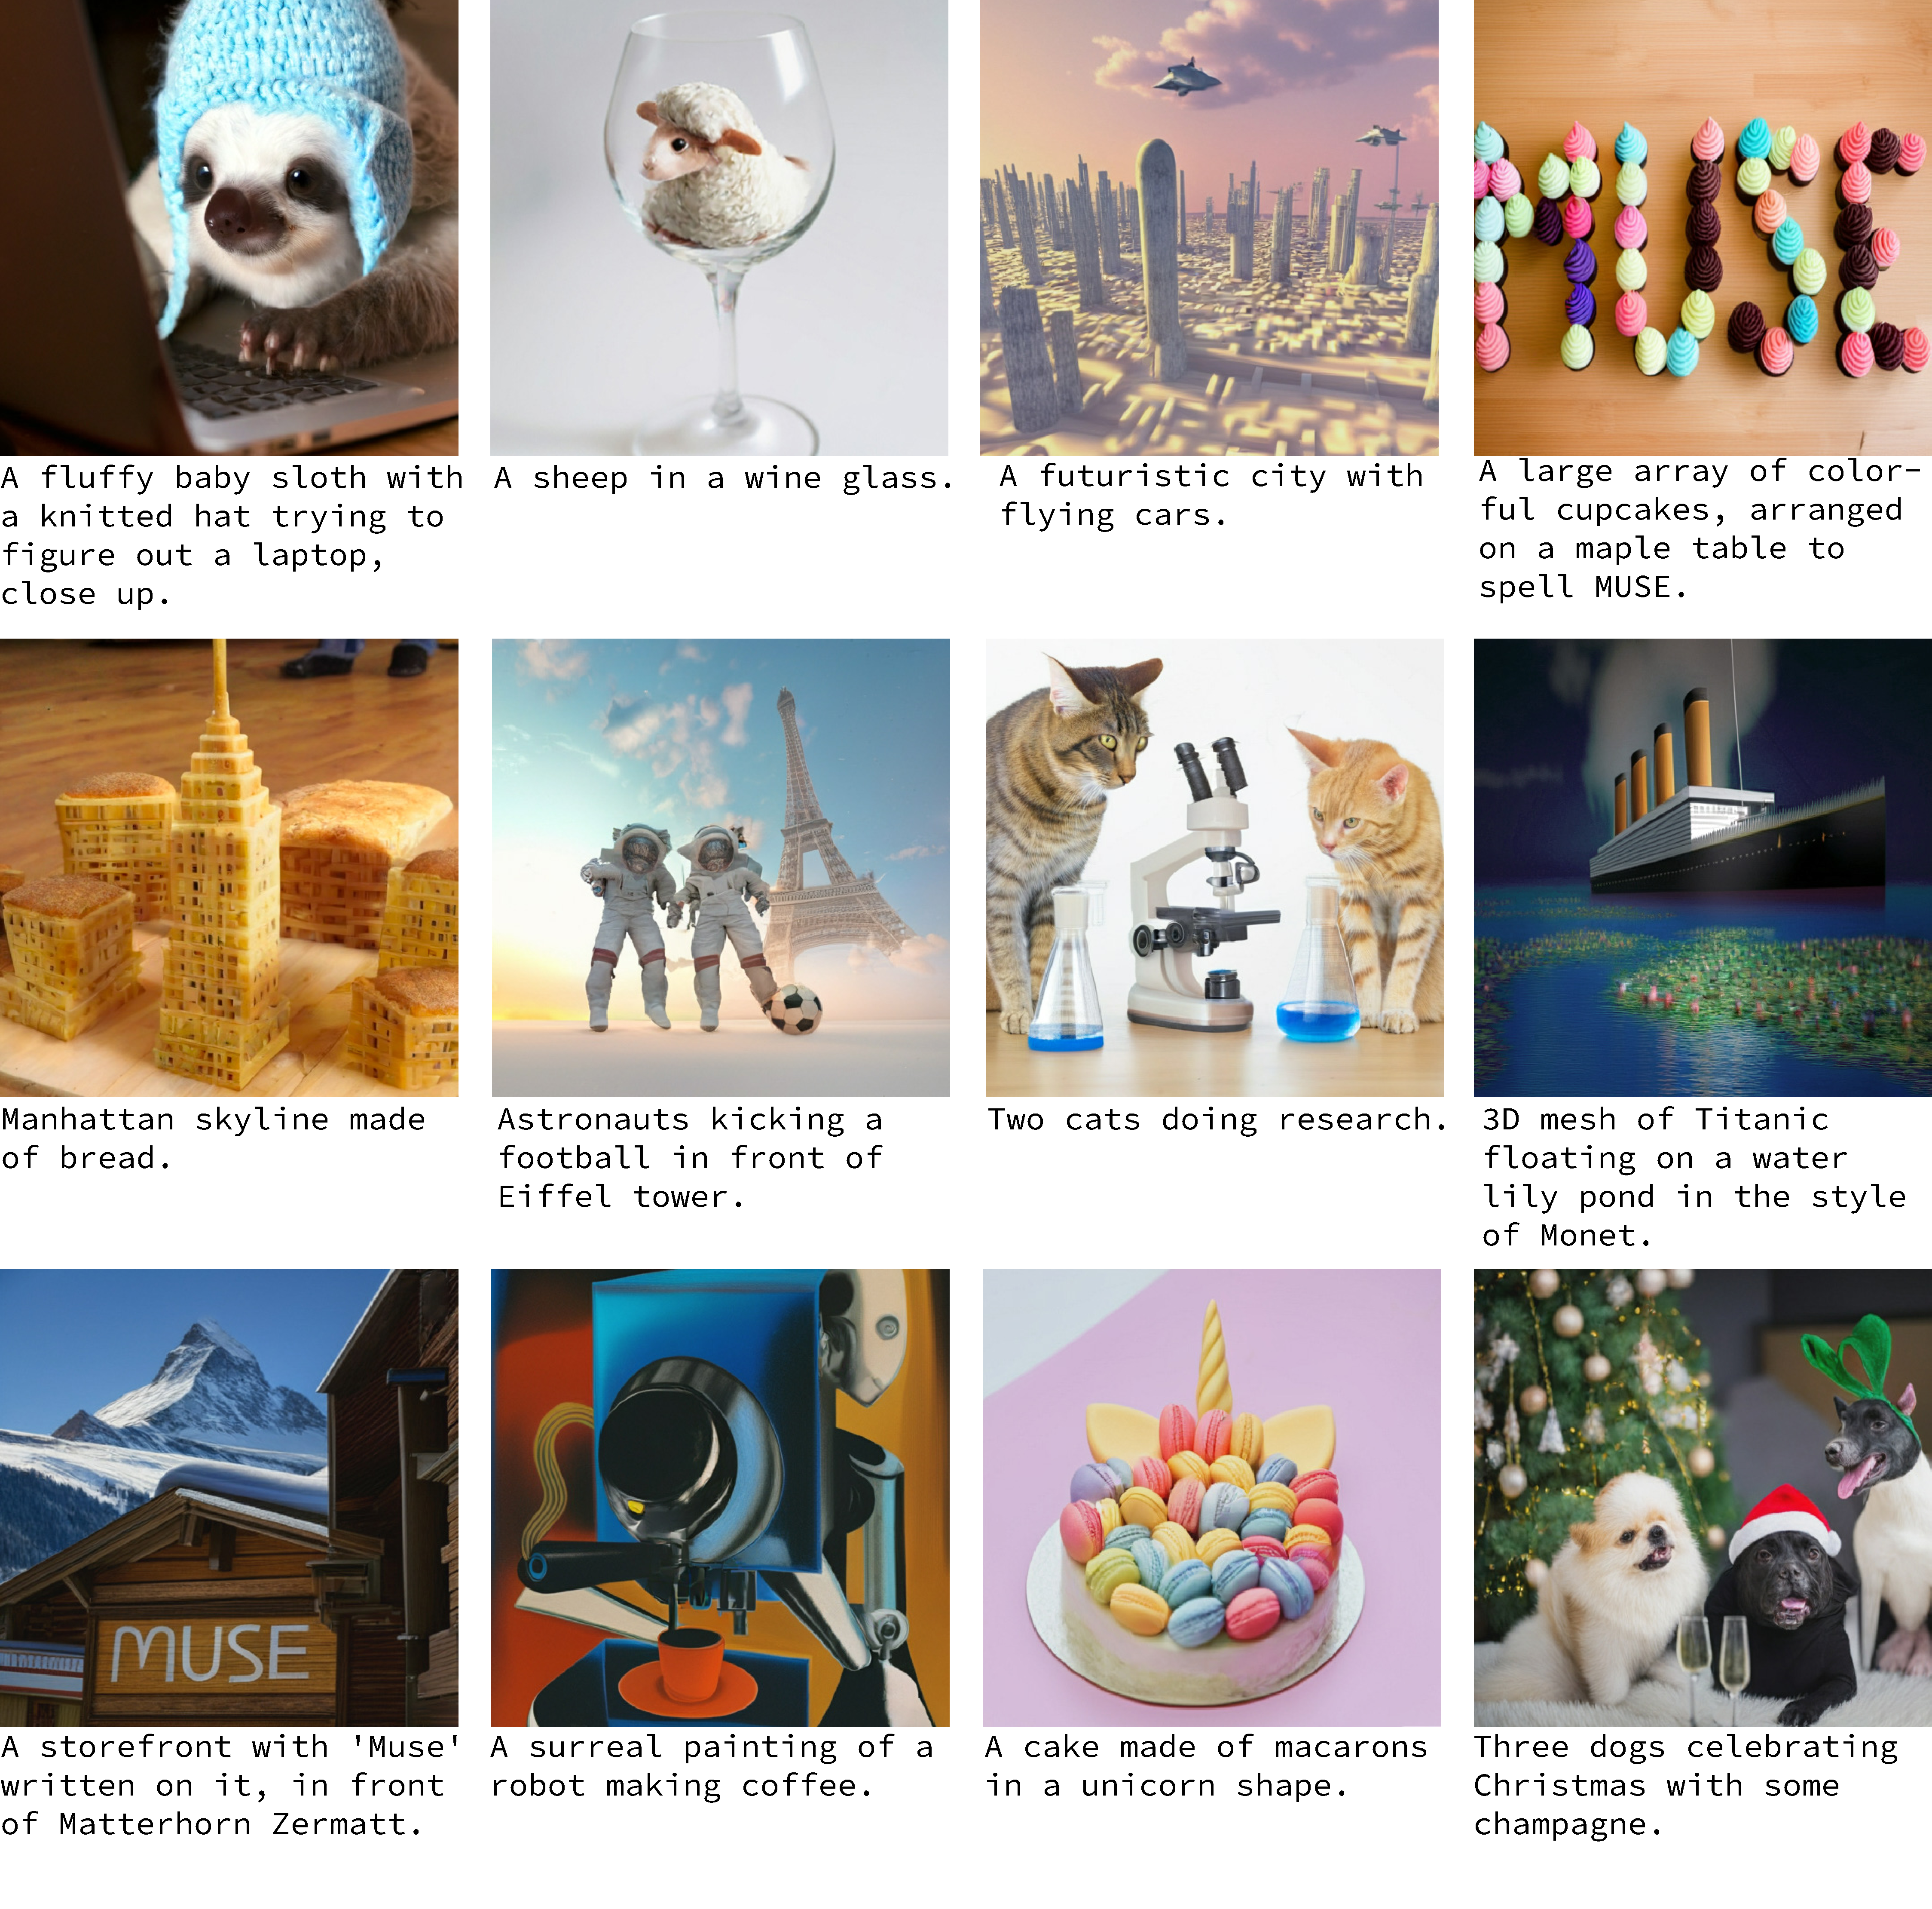
\includegraphics[width=\figwidth]{figs/teaser_v1}
% huiwen: trying to find some good substitutes
\vspace{-23pt}
\caption{\small \name~text-to-image generation ($512 \times 512$ resolution). Under each generated image, the corresponding caption is shown, exhibiting a variety of styles, captions and understanding. Each image was generated in $1.3$s on a TPUv4 chip. 
% \aj{Nit: Top middle prompt: Salvador Dali ends in an unmatched quotation.}
%Further examples are given elsewhere in the paper and at \url{\website}.
}
\label{fig:teaser_t2i}
\end{figure*}

\renewcommand{\figwidth}{1.0\textwidth}
\begin{figure*}[ht!]
% \vspace{-10pt}
\centering
\captionsetup{width=\figwidth}
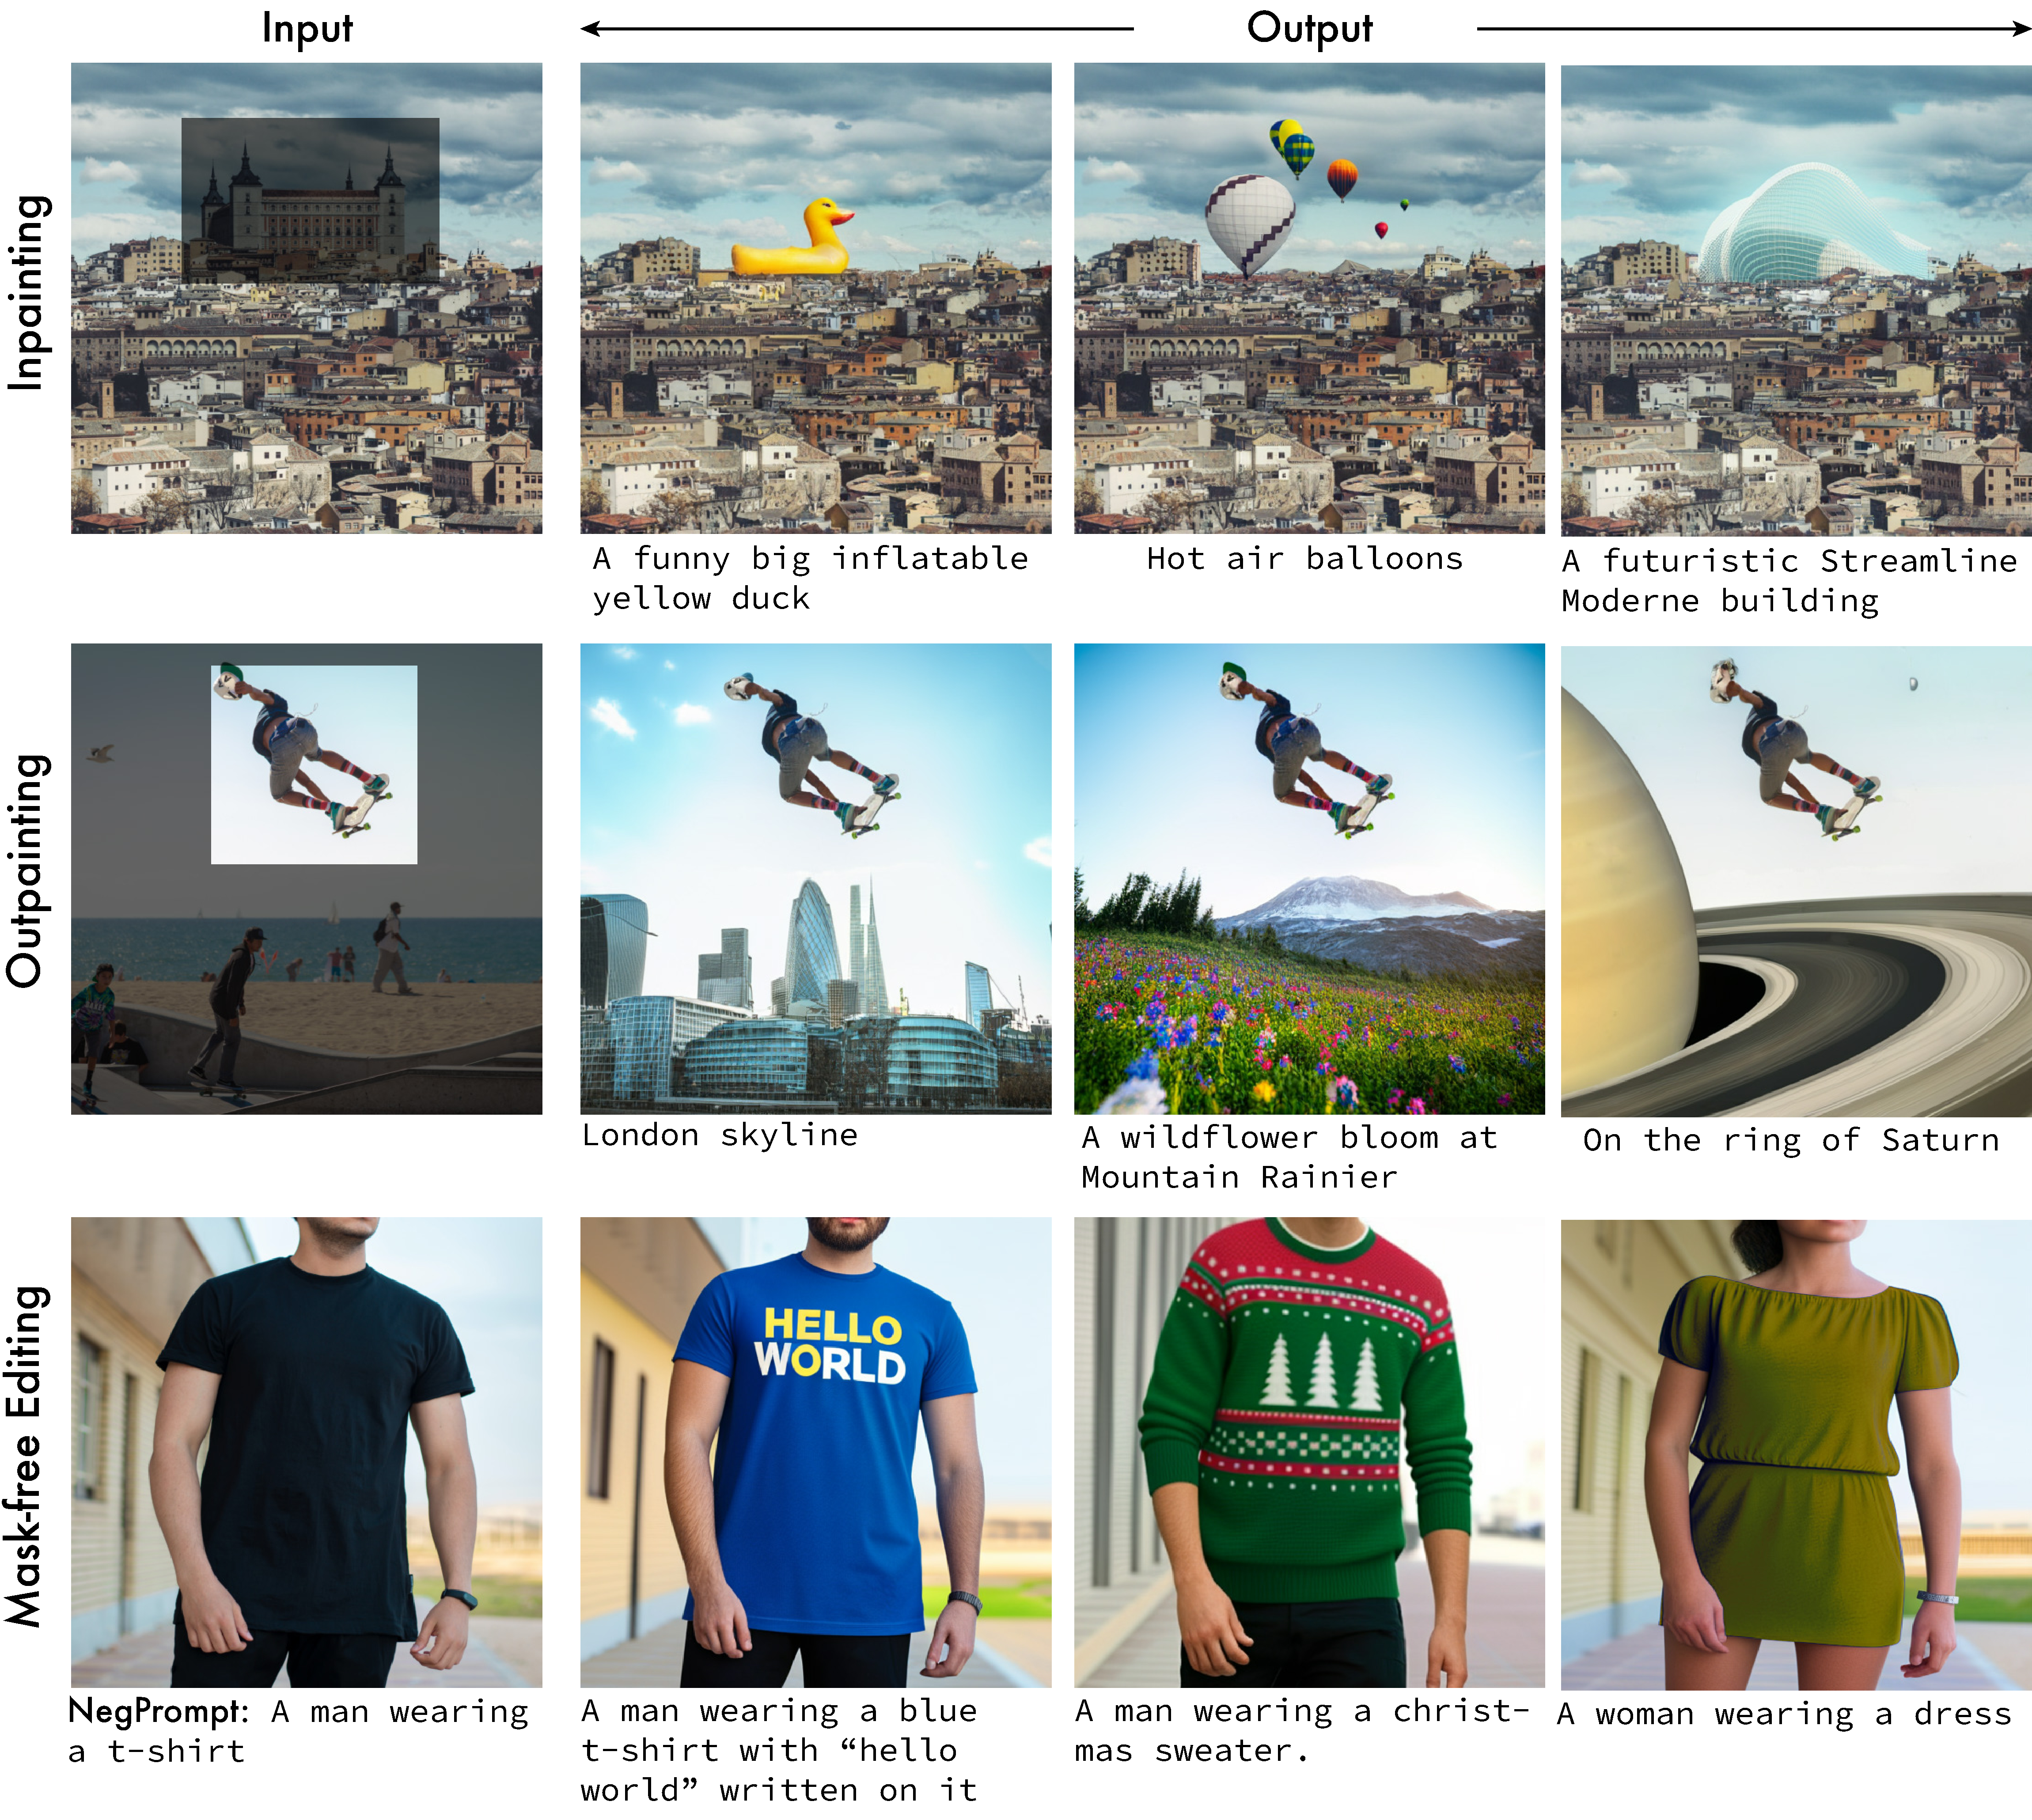
\includegraphics[width=\figwidth]{figs/teaser_editing_1}
\vspace{-18pt}
\caption{\small Examples of zero-shot text-guided image editing using \name. We show examples of a number of editing applications using the \name ~text-to-image generative model, on \emph{real} input images, without fine-tuning. All edited images are generated at $512\times512$ resolution. % \aj{``Text-guided extrapolation'' is referred to as ``Text-guided outpainting'' everywhere else in the paper.}
%Further examples are given elsewhere in the paper and at \url{\website}.
}
\vspace{-5pt}
\label{fig:teaser_edit}
\end{figure*}
